\documentclass[conference]{IEEEtran}
\IEEEoverridecommandlockouts
\usepackage{cite}
\usepackage{amsmath,amssymb,amsfonts}
\usepackage{algorithmic}
\usepackage{graphicx}
\usepackage{textcomp}
\usepackage{lipsum}
\usepackage{xcolor}
\usepackage{hyperref}
\usepackage{csquotes}
\usepackage{booktabs}
\usepackage{caption}
\usepackage{multirow} 
\usepackage{nameref}

\begin{document}

\title{Blockchain based IoT platform for smart coffee machines}

\author{
  \IEEEauthorblockN{Sebastian Kanz}
  \IEEEauthorblockA{\textit{Distributed Ledger Technologies}\\
  \textit{MaibornWolff GmbH}\\
  Frankfurt am Main, Germany\\
  sebastian.kanz@maibornwolff.de}

  \and

  \IEEEauthorblockN{Andr\'{e} Mundo}
  \IEEEauthorblockA{\textit{Distributed Ledger Technologies}\\
  \textit{MaibornWolff GmbH}\\
  Frankfurt am Main, Germany\\
  andre.mundo@maibornwolff.de}

  \and

  \IEEEauthorblockN{Michael Braun}
  \IEEEauthorblockA{\textit{Department of Computer Science}\\
  \textit{University of Applied Sciences, h\_da}\\
  Darmstadt, Germany\\
  michael.braun@h-da.de}
}

\maketitle

\begin{abstract}
Blockchain and internet of things are modern research areas with with industrial applications. Combining these relatively young and highly innovative technologies may unleash their full potential. In this paper the synergy between IoT and DLT is shown by the analyzation of a practical IoT use case and the prototypical implementation of the proposed architecture based on the blockchain platform Ethereum: Manufacturers of smart coffee machines rent their devices via a blockchain based platform to companies that enable their employees to consume coffee and pay via smartphone. Other parties like service providers or suppliers can integrate their processes and services into the platform. Payment, contract processing of e.g. rental contracts and identities are managed on-chain via smart contracts. In order to overcome the scaling problem state channels---more precisely payment channels---are utilized to enable asynchronous communication and allow offline payment. In addition, to solve the scaling problem in this use case's context it is shown that many IoT use cases require some type of asynchronicity due to device outage or connection loss. By utilization of DLT based payment channels a solution that addresses asynchronicity and scalability is proposed.
\end{abstract}

\begin{IEEEkeywords}
Blockchain, Distributed Ledger Technologies, Internet of Things, State Channel
\end{IEEEkeywords}

%
\section{Introduction}

Use cases like supply-chain tracking or new-age energy market are only a few examples of real-world \emph{blockchain} scenarios that come into touch with the \emph{Internet of Things} (IoT) where sensors and smart devices improve the acceptance and the accuracy of those use cases. On the other hand due to e.g. improved hardware capabilities and performance new IoT use cases can be implemented and concepts like smart factory or smart city can be realized. This raises the question how the two research areas might benefit from each other and which criteria or features must be fulfilled to empower DLT and IoT connected use cases.

Manufacturers of household appliances have different opportunities to sell or rent their devices not exclusively to private consumers but also to companies and the gastronomic environment. Transforming those devices into IoT devices by making them \emph{smart} with the concept of a \emph{digital twin} enables manufacturers to utilize new technology and offer new payment models and digital services to their customers. This allows the development of an ecosystem in which new business processes can emerge and several stakeholders can participate: A platform that connects those smart devices and handles the communication, data persistency, security, and the automated processing of the business logic. An evident approach for a suitable solution to create such a platform might be the application of blockchain technology---or in general the distributed ledger technology. Due to their characteristics like distribution, no-trust environment, integrity of data, and the ability of automated code-processing it is worth investigating this topic.

%
\subsection{Related work}

The goal of this article is to analyze DLTs for IoT enabler and to elaborate on DLT characteristics that empower IoT use cases. By implementing a proof-of-concept of the IoT use case based on a DLT the usability and verification of the synergies between both research areas are shown.

The topics DLT and IoT are popular research areas and there is also some work on the synergies. Research articles like~\cite{Review2018} outline possible IoT use cases that might benefit from DLTs including but not limited to the sectors health, logistics or smart cities. A more technical review on the suitability of blockchain consensus algorithms for the internet of things is done by~\cite{Salimitari2020} or \cite{Eval2018}. Similar to this work the authors of~\cite{convergence2019} describe the synergies between DLT and IoT but evaluate technical aspects like latency, throughput, and resource consumption while not distinguishing between different IoT use cases. Others like~\cite{SCIOT2016} also investigate on the meaningful application of smart contracts in IoT use cases such as this work.

In contrast to the mentioned articles that try to find a general DLT solution for the whole topic IoT this work identifies use cases and investigates this topic from a more practical view. The aim is to find a suitable solution for the use case presented in this work as well as related use cases but not cover the complete field of IoT.

%
\subsection{Pay-as-you-use renting of smart gastronomy devices}

This paper investigates the following use case (cf. Fig.~\ref{fig:overview}): Manufacturers offer their smart household appliances on a platform where customers can rent those devices and pay for the usage by a \emph{pay-as-you-use payment} model. Therefore the devices have onboard sensors which are able to track and analyze the usage and the internal machine state. To communicate with the customer and the platform the device needs interfaces like \emph{near field communication} (NFC) and access to the internet. Furthermore, stakeholders like service providers or suppliers take part on the platform and offer their services. The platform enables all parties to integrate and connect their services and business processes and offers new opportunities and use cases. The renting contracts as well as the service contracts---like the service provided by the service provider or the supply contract for supplying customers with goods---are automatically processed by the platform. This includes the communication with the devices and their onboard sensors, the payment for consuming services and goods and the information providing to the involved stakeholders. If the contract contains any conditions or time limits as well as a benefit or penalty system for involved parties this results in contract actions like value or asset transfer, contract termination, etc.

\begin{figure}[hbt]
\centering
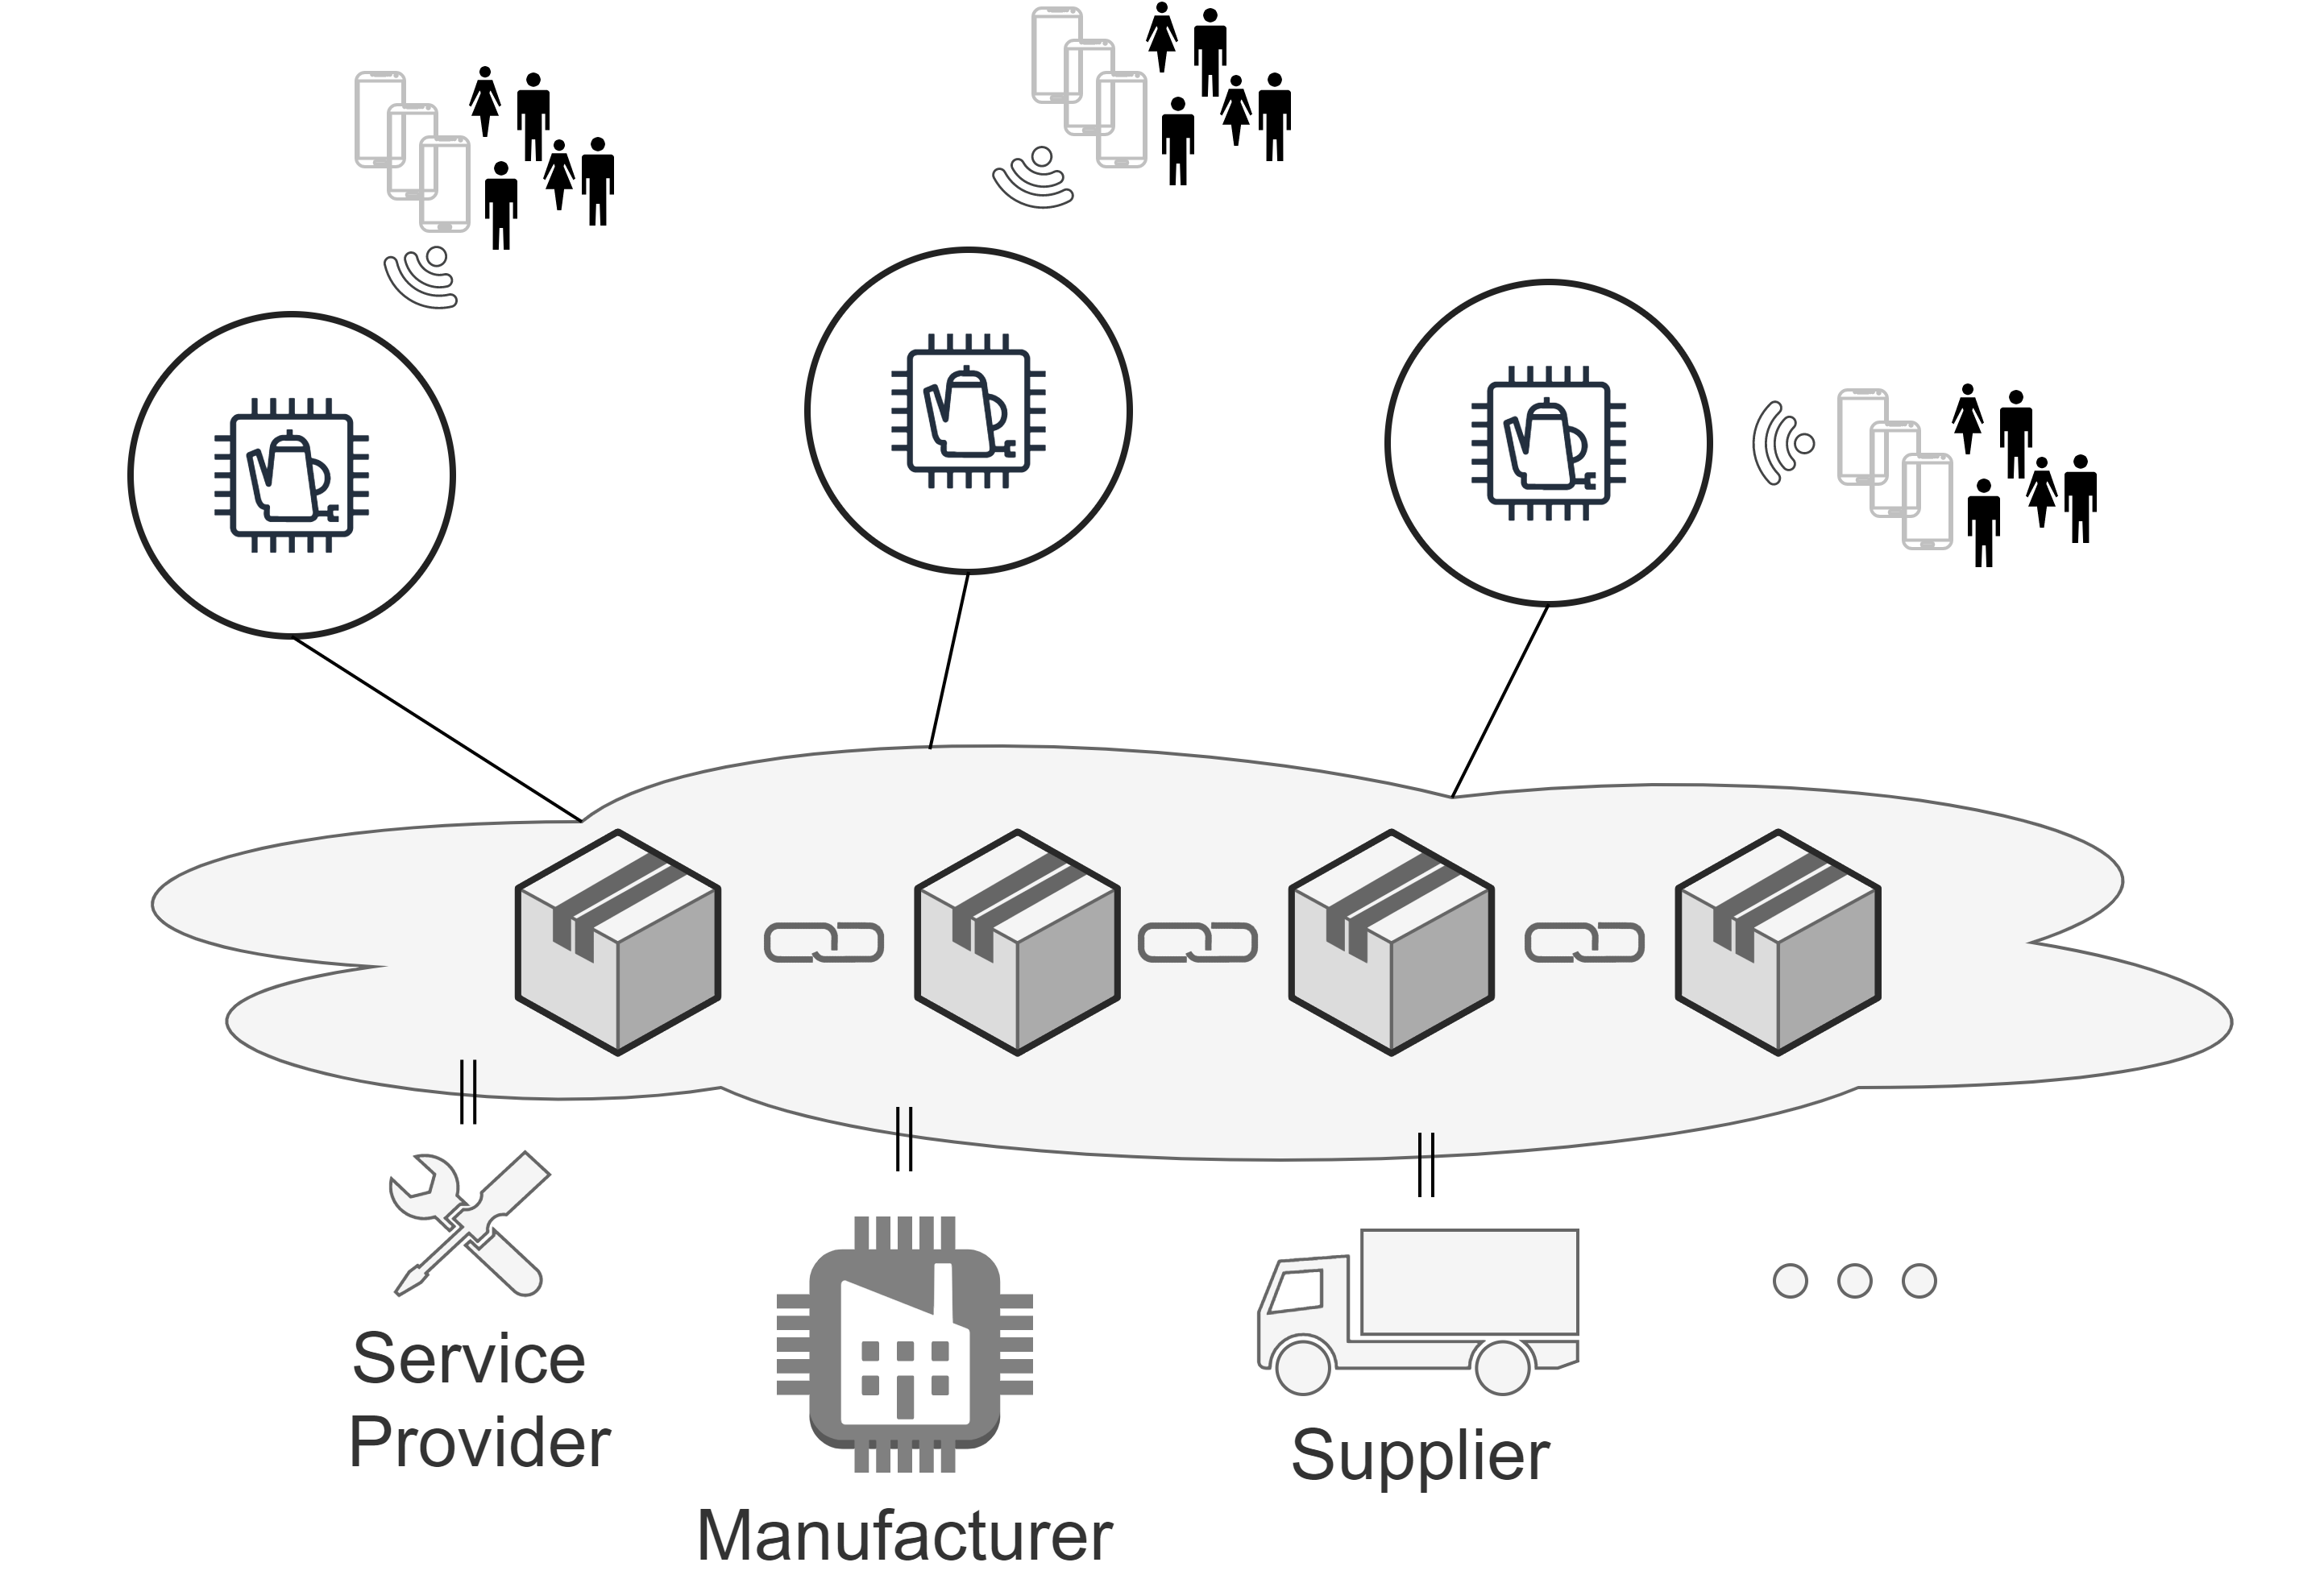
\includegraphics[width=0.5\textwidth]{overview.png}
\caption{Use case overview with involved stakeholders}
\label{fig:overview}
\end{figure}

In particular the present use case focuses on smart coffee machines rented to companies: A company---here in the role of a customer---has an active renting contract with the manufacturer. The supplier is commissioned to deliver the machine as well as optional goods to the customer. The payment and the delivery tracking are defined through the supply contract, which is processed by the platform. When the supply contract is fulfilled the supplier receives the contractually agreed value from the contract. As soon as the machine is plugged in at the customer's office and connected to the internet the employees of the customer can order their coffee. They can authorize as company employees and pay the coffee with their company-wallet via a smartphone app---the communication between their smartphone and the coffee machine is done through NFC. The coffee machine is able to check whether the company has enough credits for the coffee to be served. If the machine requires maintenance or if an error occurs the service provider is contacted. This process as well as the payment to the service provider is fully automated through the platform.

Contracts between involved parties can be setup, signed, and revoked via an UI if several conditions are met. The platform has some form of identity management to ensure that any user only acts in a specific role if he or she is allowed to. 

%
\section{Architecture}

The design and the architecture of the present use case requires the platform to implement a set of features. To find a suitable platform solution the key requirements were elaborated and transferred into the DLT context:

\begin{itemize}
\item Smart contracts allow automated information processing on-chain.
\item Oracle services provide off-chain information to the DLT.
\item Payment is needed for processing invoices of services and goods.
\item Asynchronicity empowers IoT use cases.
\item Performance is needed by every application and adjusted to the specific use case.
\item Encryption needs to be ensured to protect customer data and privacy.
\end{itemize}

\begin{table}[!htbp]
\centering
\caption{DLT selection based on key features}
\label{tab:selection}
\begin{tabular}{@{}llllll@{}}
\toprule
\multicolumn{1}{c}{} & \multicolumn{1}{c}{{\begin{tabular}[c]{@{}l@{}}Smart\\ Contracts\end{tabular}}} & \multicolumn{1}{l}{{Payment}} & \multicolumn{1}{c}{{\begin{tabular}[c]{@{}l@{}}Oracle\\ Services\end{tabular}}} & \multicolumn{1}{c}{{Async.}} & \multicolumn{1}{c}{{Encrypt.}} \\ 
\midrule
Bitcoin & (yes) & yes & (yes) & yes & no \\
BitcoinCash & (yes) & yes & (yes) & no & no \\
Corda & yes & (yes) & yes & yes & yes \\
EOS & yes & yes & yes & yes & no \\
Ethereum & yes & yes & yes & yes & yes \\
Hyperledger & yes & (yes) & yes & yes & yes \\
IOTA & no & yes & no & yes & yes \\
Quorum & yes & yes & yes & yes & yes \\
Ripple & no & yes & no & yes & no \\
Stellar & yes & yes & (yes) & yes & no \\
Tron & yes & yes & yes & yes & no \\ 
\bottomrule
\end{tabular}
\end{table}

As shown in Tab.~\ref{tab:selection}, different DLT implementations were elaborated based on the key features mentioned above. The best fitting solution seems to be Quorum, but since this implementation is directly based on Ethereum, the origin solution will be the best choice.

In the following the above mentioned features are embedded into the architectural context of the use case, which is presented in the following and described in more detail where needed. For the prototypical implementation the blockchain protocol \emph{Ethereum}~\cite{buterin2013} is used as it provides the necessary features or at least the possibility to implement them.

For the evaluation of security and encryption mechanisms for improving privacy in DLTs reference is made to~\cite{Privacy}. Those topics are evaluated in detail in the given references and are not in the focus of this paper. The integration of payment can be done via a third-party or by built-in DLT functionality like Ether or utility-tokens~\cite{Tokens}.

An important concept that needs to be mentioned is the smart contract which enables this use case to be fully automated and process contracts and contract logic on-chain as well as providing oracle services. Due to the fact that most modern DLTs offer smart contract functionality this topic is not investigated on in detail. The key concept that empowers this use case is asynchronous communication and information processing. Most IoT use cases have too few resources for providing user-friendly synchronous communication. Due to connection-loss, power-outage or less computing resources IoT devices cannot guarantee a constant communication channel to other devices. Pushing the concept of asynchronicity a little further and increasing the timeout between connections leads to the notion of \emph{offline capability}. To be able to offer the customers a satisfying user-experience the most critical point is the user interaction---in this use case namely the serving of the coffee. If this process takes too long or aborts due to errors the customers decline the use case and the acceptance decreases as well as the economic efficiency.

Therefore, the technology of the underlying platform needs a mechanism for this offline functionality: The processing, the payment, and the synchronization needs to take place in different time intervals. DLTs as a possible modern solution offer so-called \emph{state channels} to tackle this issue. With offline communication, hashing and signing algorithms, and the utilization of smart contracts DLTs can ensure security, data integrity, and payment processing in this scenario. The concept of state-channels is examined in detail in the following section.

%
\subsection{Excursus: State channels for empowering and scaling IoT use cases}

Blockchains are a compromise due to their nature. Due to the consensus protocol---independent of block size and network capacity---a natural limit is given: For example, the Bitcoin network~\cite{nakamoto2009} is limited on a block time of 10 minutes by the complex calculation of Proof-of-Work (PoW). If the block size is very small blocks are propagated very quickly over the network but only a few transactions can be transferred at once. If the block size is very large it is very difficult for nodes to synchronize but more transactions can be transferred at once. This limitation of block size and block duration means that in the case of Bitcoin currently (as of 01/2020) on average about 7 transactions per second are possible~\cite{Macdonald2017}.

Other implementations may use other consensus mechanisms and other parameters but there are also natural barriers there. It becomes clear that with increasing demand mainly for the transaction processing per time interval (mostly transactions per second (TPS)) an improved performance and new solutions become necessary~\cite{Macdonald2017}. As a possible answer to the scaling problem of blockchains so-called state channels were developed. The aim is to be able to transmit any kind of off-chain processing of status-changing operations which are typically processed and stored on-chain. Thus the number of transactions can be reduced and the interaction time between involved parties can be improved. In the context of payments, so-called micro-payments are made possible. State channels which are limited to payment processing are called payment channels. These can be faster and cheaper than normal transactions take place. The costs of such micro-payments can be kept very low, since not all transactions must be stored on-chain~\cite{Coleman2018}

Another big advantage of state channels is the empowerment of asynchronous transactions. If participants are not in the blockchain network (e.g. due to connectivity problems) then no transactions are carried out. If real-world actions like the opening of a barrier or the processing of an action are dependent from an on-chain status update then with loss of connectivity the real process stands still until the connection is restored. State-channels could be used here in order to create an alternative processing that can also be used when the blockchain is not reachable. Examples of an implementation of state channels are Bitcoin's Lightning Network~\cite{Lightning2016}, Ethereum's Raiden Network or the implementation of Neo called Trinity~\cite{Trinity2018}.

%
\subsection{Asynchronous payment processing}

The payment-channels in the present use case are a practical realization of one-way payment-channels for IoT devices and they are implemented as smart contracts on the Ethereum blockchain. When a user submits to a rental offering and the renting contract is created the corresponding smart contract creates the data structure on-chain and initializes a payment agreement that is designed by a separate smart contract. This creates the payment-channel between the involved parties and holds all relevant data.

Initially the payment-channel between the coffee machine and the customer is charged with a predefined amount of credits transferred on contract creation. The payment-channel is implemented as a one-way payment-channel since the value is exchanged only to the wallet of the machine. Credits that remain in the channel after the machine closes the channel will be transferred back to the customer. Apart from the general concept of payment-channels the present one implements a redeem function that pays out the transferred credits the receivers. Due to this functionality the payment-channels can be reused and recharged and do not need to be recreated; this is for performance and cost issues.

While the payment agreement data structure is an on-chain information container for the payment-channel the communication between the participants happens off-chain. The data is only needed for data persistency purposes and for synchronization of the participants. To be able to transfer data from the coffee machines to the employees and back there must be a communication channel besides the blockchain. This is implemented by exchanging data via NFC: After pressing the coffee serving button, the coffee machine sends the payment data as a receipt via NFC to the employee's smartphone. The data is signed with the employee's private key and sent back from the smartphone to the coffee machine. The machine is able to verify the signature and persists the latest receipt locally. This process can be repeated as many times as there are enough credits in the payment-channel. Because there might occur a connection-loss the coffee machine might not be able to check the balance on-chain and has to rely on its local information. Since the payment-channels are one-way there is no possibility for the customer to pay out his own credits and to order a new coffee while the machine is offline. This must be ensured to avoid data inconsistency. If the balance of the payment-channel reaches a critical threshold or a defined time interval is reached the machine redeems the receipts and the money is transferred on-chain. The customer---in this use case the company or an authorized employee---can charge the payment-channel again to order more coffee in the future.

The described payment process with the utilization of the payment-channel as part of the renting agreement can be transferred to the other payment processes between more stakeholders like the service provider mentioned above. The base concept and implementation remain the same.

%
\subsection{Identity verification an privacy aspects}

Another important part of the use case is the identity management and verification of the participating users. It is necessary that each user acts in a well-defined role as this information is important to use case itself: For example, a coffee machine should only be allowed to trigger certain tasks while only manufacturers should be able to administer their machines. For that reason an on-chain smart contract acting as an oracle service is implemented. During an onboarding process, e.g. the registering on the platform the user is identified and assigned a role which is persisted in that smart contract. The owner of the smart contract is able to maintain the data as well as adding new roles and identities. To make this approach more decentralized many owners could be possible in future. The administrative tasks could be commissioned by a vote system.

The present implementation does not focus on privacy concerns as they do not belong to the key functionality and can be implemented later. Nevertheless, privacy is an important topic to be investigated when it comes to a real world adoption. Some privacy vulnerabilities are listed below without claiming to be complete:

\begin{itemize}
\item Third parties are able to track the coffee consumption per customer account. Due to the fact, that in the current implementation an account is used by all employees of an office, no assertion can be made for a single person. The consumption is not related to a single day but to a period of time.
\item Information of costs, usage, and contract periods are visible to third parties.
\item Third parties can determine the role of an account whether it acts as a machine, a customer, a manufacturer or another role.
\end{itemize}
Those vulnerabilities can be avoided through the utilization of techniques like the Zerocoin protocol~\cite{zerocoin2013} or providing another identity management solution than an on-chain smart contract. In the context of the present proof of concept, the on-chain solution was preferred because of the easy integration.

%
\subsection{Architectural overview of involved components}

The present use case has been evaluated by a prototypical implementation with the Ethereum blockchain. The focus has been laid on the general feasibility and the synergy between DLT and IoT. 

\begin{figure*}[hbt]
\centering
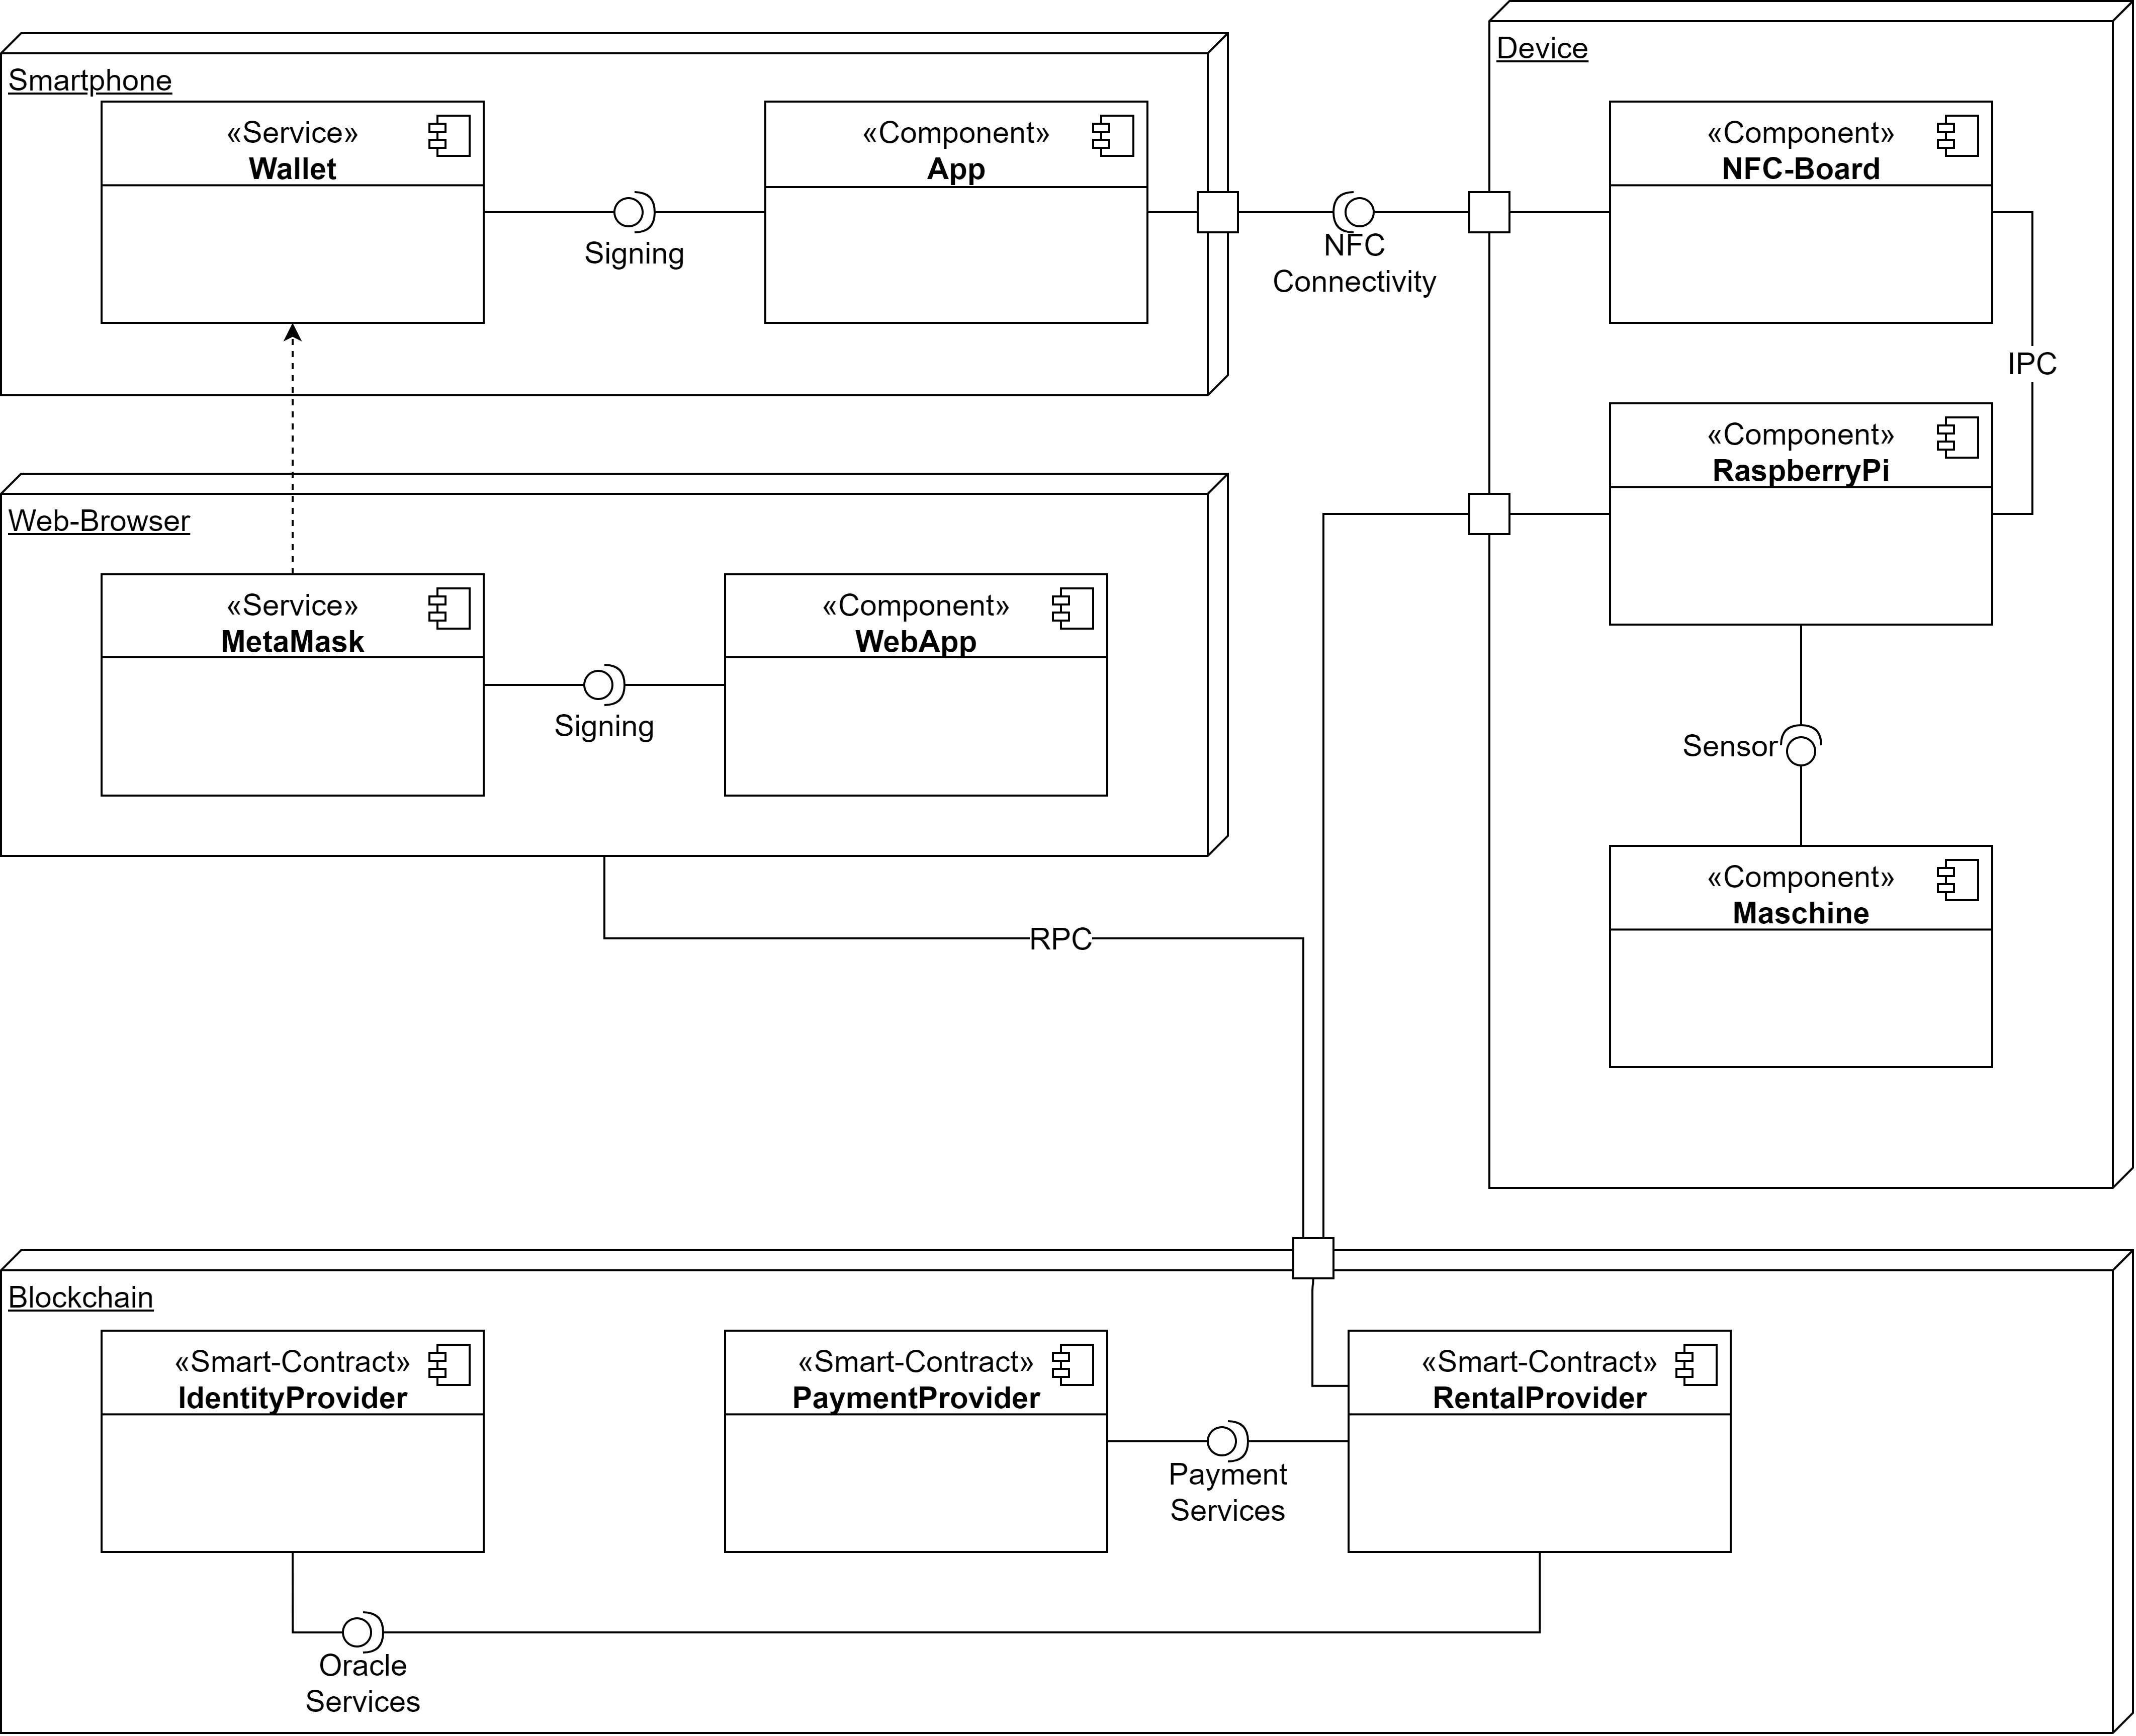
\includegraphics[width=1.0\textwidth]{Architecture.png}
\caption{UML components diagram; architectural overview}
\label{fig:architecture}
\end{figure*}

An overview of the application's architecture is shown in Fig.~\ref{fig:architecture}. On-chain information is processed and stored via three smart contracts: The IdentityProvider takes care of the contracting parties and manages access control. The PaymentProvider holds the payment-channels for the renting contracts and handles payment processing. The RenalProvider models the rental contracts on-chain and controls and calls the other smart contracts.

Information on rentable devices, active contracts, contract handling and payment is accessible by all participants through a web app. The browser-integrated wallet MetaMask is used to sign and verify transactions to and from the blockchain.

To interact with the coffee machine the customer needs a smartphone with enabled NFC service. A mobile app enables the customer to authorize payments and sign incoming receipts from the coffee machine via NFC. The wallet used on the smartphone is the same as the one in the browser, so all information and contracting can be done across device boundaries.

To upgrade coffee machines and make them smart (as long as they do not support smart functionality out of the box) a RaspberryPi mini-computer is used in conjunction with a NFC breakout-board. This board is used for communication between the coffee machine and the smartphone. To measure the internal device state and gather usage data the device needs onboard sensors which must be available for the RaspberryPi to call (e.g. via REST or hardware-near protocols like I2C). The RaspberryPi itself can call the blockchain to redeem the receipts or to report errors or request service inquiry.

%
\section{Results}

With the successful implementation of this use case the general feasibility is shown. The following subsections examine different aspects in detail.

%
\subsection{Performance}

The performance from the user's point of view must be divided into two phases of use: The initial contract creation is an asynchronous process that requires the intervention of both contract parties and therefore cannot be measured exactly. If this process is transferred to the analog process---the contract request until the conclusion of the contract---a significant increase in speed can be observed through digitalization of that process. The processing time from the request to the conclusion of the contract corresponds to three on-chain transactions and thus lasts on average only a few minutes. The actual usage, i.e. the interaction of the user with the coffee machine, is instantaneous and offers the user optimal performance and thus a good user experience. From the manufacturer's point of view, there are no time-critical processes, as it is not important that a contract is concluded within seconds, as the time at which the customer confirms the contract cannot be affected. A receipt can be cashed out with one on-chain transaction within a few seconds (less than a minute) and is therefore within an acceptable time frame. 

%
\subsection{Security}

The use case is based on a role and user management system which checks permissions and restricts access. The central security aspect is the private key of every user. Currently there exists no implemented mechanism to prevent the loss or theft of the private key. Furthermore, the certification of users as a company's employee is currently rudimentarily implemented and can be improved by utilizing verifiable credentials and decentralized identifiers in that context.

Due to its distributed and distrusting nature the blockchain can be seen as a secure environment; manipulations or attacks on the system are only possible with high effort and immense costs. Possible attack vectors are outlined in~\cite{EthereumSecurity} and~\cite{BlockchainSecurity}. Nevertheless, the security of the implemented smart contracts must be audited by experts before a go-live to a productive environment so that damages caused by third parties or errors in the code can be avoided.

%
\subsection{Operating costs}

The use case is calculated as an industry-realistic quantity structure for the German market based on customer experience of MaibornWolff GmbH. The following numbers and data are based on the tests from the prototype or marked as assumptions.

A final configuration level of the present use case might include a total of 10,000 coffee machines on rent and 40 employees per office on average as well as a per capita consumption per year of coffee 164 litres. At the time of calculating the Ethereum price was at 196.04 EUR per 1 ETH; the GAS price is set to 5 GWEI. A more detailed overview of the assumptions made and the underlying data is shown in the \nameref{appendix}.

%
\section{Conclusion}

The implementation of the pay-as-you-use renting use case of smart coffee machines based on the Ethereum blockchain has been successful. It prototypically evaluates the suitability of DLTs for the IoT use case by utilizing payment channels of Ethereum's smart contracts for fulfilling the need for asynchronicity.

Due to the diversity of the topic IoT, a general statement for the entire IoT application area is thus not made and cannot be fully validated. Use cases that show similar characteristics as the present implementation can profit with a high degree of certainty from a DLT implementation and the associated advantages. On the other hand, time-critical or performance-heavy IoT applications cannot be implemented on the basis of a DLT because, for example, the required real-time communication is not available. In addition, applications that affect only a single stakeholder or are only executed at a single location are not designed for DLTs either, as they cannot benefit from the decentralized and no-trust environment.

It is shown that the suitability of DLTs for IoT use cases from the performance perspective is a tradeoff between on-chain state replication where all data is stored on the blockchain and can be reproduced and off-chain communication via state channels. For similar use cases the question must be answered how long a state channel can be kept open without syncing with the blockchain. The more this time can be increased the less performance is required due to increased asynchronicity in the IoT use case and the easier it can be implemented in DLTs. If possible this time window should be increased as much as possible provided that the user experience does not suffer from that. On the other hand the downside of those time gaps in such use cases must be considered, e.g. the delayed asset or value transfer. 

%
\section{Future Work}

As possible improvements of the shown use case two approaches will be pointed out below.

Privacy is an important topic that was not intentionally not implemented in detail in this proof of concept as it was not in the focus of the work. Nevertheless, to implement a market-ready IoT use case this topic must be addressed as much as possible to offer a good and secure user-experience. A possible approach and a current research topic are so-called zero knowledge proofs. Without going into detail, a provider of such a proof can show the possessing of a secret (e.g. the birth date) and reveal that a certain information is true (e.g. to be old enough to buy alcohol) without sharing the secret with the requester. The requesting entity can check and verify the proof mathematically. With that technique, privacy can be improved in that use case e.q. by replacing the on-chain identity smart contract. Further research in this area might show more potential.

On the other side the costs of an industry use case like the one shown in this paper is a relevant factor to consider. To further reduce the costs, one approach might be the outsourcing of on-chain saved data to the off-chain world (e.g. like IPFS), because on-chain data storage is expensive. As IPFS and similar solutions are still under heavy development, there might be a suitable solution to improve this use case.


\section*{Acknowledgment}
This research was supported by the distributed ledger technology department of MaibornWolff GmbH, Frankfurt, and the department for computer science of the University of Applied Sciences (h\_da), Darmstadt. We thank the colleagues for providing their expertise and for assisting the research.

% Generated by IEEEtran.bst, version: 1.12 (2007/01/11)
\begin{thebibliography}{10}
\providecommand{\url}[1]{#1}
\csname url@samestyle\endcsname
\providecommand{\newblock}{\relax}
\providecommand{\bibinfo}[2]{#2}
\providecommand{\BIBentrySTDinterwordspacing}{\spaceskip=0pt\relax}
\providecommand{\BIBentryALTinterwordstretchfactor}{4}
\providecommand{\BIBentryALTinterwordspacing}{\spaceskip=\fontdimen2\font plus
\BIBentryALTinterwordstretchfactor\fontdimen3\font minus
  \fontdimen4\font\relax}
\providecommand{\BIBforeignlanguage}[2]{{%
\expandafter\ifx\csname l@#1\endcsname\relax
\typeout{** WARNING: IEEEtran.bst: No hyphenation pattern has been}%
\typeout{** loaded for the language `#1'. Using the pattern for}%
\typeout{** the default language instead.}%
\else
\language=\csname l@#1\endcsname
\fi
#2}}
\providecommand{\BIBdecl}{\relax}
\BIBdecl

\bibitem{Review2018}
T.~M. {Fern\'{a}ndez-Caram\'{e}s} and P.~{Fraga-Lamas}, ``{A Review on the Use
  of Blockchain for the Internet of Things},'' \emph{IEEE Access}, vol.~6, pp.
  32\,979--33\,001, 2018.

\bibitem{Salimitari2020}
\BIBentryALTinterwordspacing
M.~Salimitari, M.~Chatterjee, and Y.~Fallah, ``{A Survey on Consensus Methods
  in Blockchain for Resource-constrained IoT Networks},'' 4 2020. [Online].
  Available:
  \url{https://www.techrxiv.org/articles/preprint/A_Survey_on_Consensus_Methods_in_Blockchain_for_Resource-constrained_IoT_Networks/12152142}
\BIBentrySTDinterwordspacing

\bibitem{Eval2018}
R.~Han, V.~Gramoli, and X.~Xu, ``{Evaluating Blockchains for IoT},'' in
  \emph{9th IFIP International Conference on New Technologies, Mobility and
  Security (NTMS), 2018}, 2018, pp. 1--5.

\bibitem{convergence2019}
\BIBentryALTinterwordspacing
M.~Maroufi, R.~Abdolee, and B.~Tazekand, ``{On the Convergence of Blockchain
  and Internet of Things (IoT) Technologies},'' \emph{Journal of Strategic
  Innovation and Sustainability}, vol.~14, no.~1, 2019. [Online]. Available:
  \url{https://www.articlegateway.com/index.php/JSIS/article/view/990}
\BIBentrySTDinterwordspacing

\bibitem{SCIOT2016}
K.~Christidis and M.~{Devetsikiotis}, ``{Blockchains and Smart Contracts for
  the Internet of Things},'' \emph{IEEE Access}, vol.~4, pp. 2292--2303, 2016.

\bibitem{buterin2013}
\BIBentryALTinterwordspacing
V.~Buterin, ``{Ethereum: A Next-Generation Smart Contract and Decentralized
  Application Platform},'' 2013. [Online]. Available:
  \url{https://github.com/ethereum/wiki/wiki/White-Paper}
\BIBentrySTDinterwordspacing

\bibitem{Privacy}
A.~{Unterweger}, F.~{Knirsch}, C.~{Leixnering}, and D.~{Engel}, ``Lessons
  learned from implementing a privacy-preserving smart contract in ethereum,''
  pp. 1--5, 2018.

\bibitem{Tokens}
M.~Di~Angelo and G.~Salzer, ``Tokens, Types, and Standards: Identification and
  Utilization in Ethereum,'' 03 2020.

\bibitem{nakamoto2009}
\BIBentryALTinterwordspacing
S.~Nakamoto, ``{Bitcoin: A Peer-to-Peer Electronic Cash System},'' 2009.
  [Online]. Available: \url{http://www.bitcoin.org/bitcoin.pdf}
\BIBentrySTDinterwordspacing

\bibitem{Macdonald2017}
M.~Macdonald, L.~Liu-Thorrold, and R.~Julien, ``{The Blockchain: A Comparison
  of Platforms and Their Uses Beyond Bitcoin},'' 02 2017.

\bibitem{Coleman2018}
\BIBentryALTinterwordspacing
J.~Coleman, L.~Horne, and L.~Xuanji, ``{Counterfactual: Generalized State
  Channels},'' 2018. [Online]. Available:
  \url{http://l4.ventures/papers/statechannels.pdf}
\BIBentrySTDinterwordspacing

\bibitem{Lightning2016}
\BIBentryALTinterwordspacing
J.~Poon and T.~Dryja, ``{The Bitcoin Lightning Network: Scalable Off-Chain
  Instant Payments},'' 2016. [Online]. Available:
  \url{https://lightning.network/lightning-network-paper.pdf}
\BIBentrySTDinterwordspacing

\bibitem{Trinity2018}
\BIBentryALTinterwordspacing
J.~XU, Z.~Ji, and Y.~Li, ``{An Off-chain Scaling Solution for Neo},'' 2018.
  [Online]. Available: \url{https://trinity.tech/#/writepaper}
\BIBentrySTDinterwordspacing

\bibitem{zerocoin2013}
I.~Miers, C.~Garman, M.~Green, and A.~D. Rubin, ``{Zerocoin: Anonymous
  Distributed E-Cash from Bitcoin},'' in \emph{2013 IEEE Symposium on Security
  and Privacy}, 2013, pp. 397--411.

\bibitem{EthereumSecurity}
\BIBentryALTinterwordspacing
H.~Chen, M.~Pendleton, L.~Njilla, and S.~Xu, ``A Survey on Ethereum Systems
  Security: Vulnerabilities, Attacks, and Defenses,'' New York, NY, USA, Jun.
  2020. [Online]. Available: \url{https://doi.org/10.1145/3391195}
\BIBentrySTDinterwordspacing

\bibitem{BlockchainSecurity}
J.~{Moubarak}, E.~{Filiol}, and M.~{Chamoun}, ``{On Blockchain Security and
  Relevant Attacks},'' pp. 1--6, 2018.

\end{thebibliography}


\newpage

\section*{Appendix}
\label{appendix}

\begin{table}[!htbp]
\centering
\caption{DLT selection based on key features}
\begin{tabular}{llll}
\textbf{Description}                         & \textbf{Amount}     & \textbf{Unit}                                                 & \textbf{}                                                           \\
GAS price                                    & 5                   & GWEI                                                          &                                                                     \\
ETH price                                    & 196.04              & Euro                                                          &                                                                     \\
Number of coffee machines                    & 10,000              & Machines                                                      & (assumption)                                                        \\
Employees per coffee machine                 & 40                  & Employees                                                     & (assumption)                                                        \\
Total employees                              & 400,000             & Employees                                                     &                                                                     \\
Liter of coffee per year per person          & 164                 & Liter                                                         &                                                                     \\
Cups of coffee (0,2l) per year               & 820                 & Cups                                                          &                                                                     \\
Working days (less 30 days holiday)          & 230                 & Days                                                          &                                                                     \\
Cups of coffee (0,2l) per day                & 2.24                & Cups                                                          &                                                                     \\
Prepaid credit sufficient for                & 5                   & \begin{tabular}[c]{@{}l@{}}Days\\ (Working week)\end{tabular} &                                                                     \\
Price per cup of coffee                      & 0.25                & Euro                                                          & (assumption)                                                        \\
\textbf{Sales volume per machine and week}   & \textbf{157,69}     & \textbf{Euro}                                                 &                                                                     \\
Prepaid credit to be topped up per machine   & 200                 & Euro                                                          & \begin{tabular}[c]{@{}l@{}}(assumption,\\ plus buffer)\end{tabular} \\
\textbf{Total turnover (annual)}             & \textbf{82,000,000} & \textbf{Euro}                                                 &                                                                     \\
\textbf{Total turnover per machine (annual)} & \textbf{8,200}      & \textbf{Euro}                                                 & \multicolumn{1}{c}{\textbf{}}                                      
\end{tabular}
\end{table}


\begin{table}[!htbp]
\centering
\caption{DLT selection based on key features}
\begin{tabular}{clllll}
\textbf{}                     & \multicolumn{1}{c}{\textbf{}}            & \multicolumn{4}{c}{\textbf{Individual costs}}                                                                                              \\
\textbf{Sender}               & \multicolumn{1}{c}{\textbf{Transaction}} & \multicolumn{1}{c}{\textbf{GAS}} & \multicolumn{1}{c}{\textbf{WEI}} & \multicolumn{1}{c}{\textbf{ETH}} & \multicolumn{1}{c}{\textbf{Euro}} \\
\multirow{2}{*}{Manufacturer} & Contract creation                        & 426,609                          & 2,133,045                        & 0.002133                         & 0.42                              \\
                              & Redeem receipt                           & 157,927                          & 789,635                          & 0.00079                          & 0.15                              \\
\multirow{3}{*}{Customer}     & Request contract                         & 197,964                          & 989,820                          & 0.00099                          & 0.19                              \\
                              & Accept contract                          & 162,743                          & 813,715                          & 0.000814                         & 0.16                              \\
                              & Charge prepaid                           & 28,805                           & 144,025                          & 0.000144                         & 0.03                             
\end{tabular}
\end{table}


\begin{table}[!htbp]
\centering
\caption{DLT selection based on key features}
\begin{tabular}{lcrccrc}
\multicolumn{1}{c}{\textbf{}}            & \textbf{\begin{tabular}[c]{@{}c@{}}Transactions\\ per machine\\ (one-time)\end{tabular}} & \multicolumn{1}{c}{\textbf{\begin{tabular}[c]{@{}c@{}}Transaction costs\\ per machine\\ (one-time)\end{tabular}}} & \textbf{\begin{tabular}[c]{@{}c@{}}Transaction consts\\ of all machines\\ (one-time)\end{tabular}} & \textbf{\begin{tabular}[c]{@{}c@{}}Transactions\\ per machine\\ \\ (annually)\end{tabular}} & \multicolumn{1}{c}{\textbf{\begin{tabular}[c]{@{}c@{}}Transaction costs\\ per machine\\ (annually)\end{tabular}}} & \textbf{\begin{tabular}[c]{@{}c@{}}Transaction costs\\ of all machines\\ (annually)\end{tabular}} \\
\multicolumn{1}{c}{\textbf{Transaction}} & \textbf{Amount}                                                                          & \multicolumn{1}{c}{\textbf{Euro}}                                                                                 & \textbf{Euro}                                                                                      & \textbf{Amount}                                                                             & \multicolumn{1}{c}{\textbf{Euro}}                                                                                 & \textbf{Euro}                                                                                     \\
Contract creation                        & 1                                                                                        & \textbf{0,42}                                                                                                     & \multicolumn{1}{r}{\textbf{4.200,00}}                                                              & 0                                                                                           & \textbf{0,00}                                                                                                     & \multicolumn{1}{r}{\textbf{0,00}}                                                                 \\
Redeem receipt                           & 0                                                                                        & \textbf{0,00}                                                                                                     & \multicolumn{1}{r}{\textbf{0,00}}                                                                  & 52                                                                                          & \textbf{7,80}                                                                                                     & \multicolumn{1}{r}{\textbf{78.000,00}}                                                            \\
Request contract                         & 1                                                                                        & \textbf{0,19}                                                                                                     & \textbf{--}                                                                                         & 0                                                                                           & \textbf{0,00}                                                                                                     & \textbf{--}                                                                                        \\
Accept contract                          & 1                                                                                        & \textbf{0,16}                                                                                                     & \textbf{--}                                                                                         & 0                                                                                           & \textbf{0,00}                                                                                                     & \textbf{--}                                                                                        \\
Charge prepaid                           & 0                                                                                        & \textbf{0,00}                                                                                                     & \textbf{--}                                                                                         & 41                                                                                          & \textbf{1,23}                                                                                                     & \textbf{--}                                                                                       
\end{tabular}
\end{table}


\end{document}
